\documentclass[tikz]{standalone}
\usepackage{xcolor}
\usetikzlibrary{arrows.meta}

\def\range{9}
\def\xyRatio{2/3}
\def\circSize{1.2mm}

\begin{document}
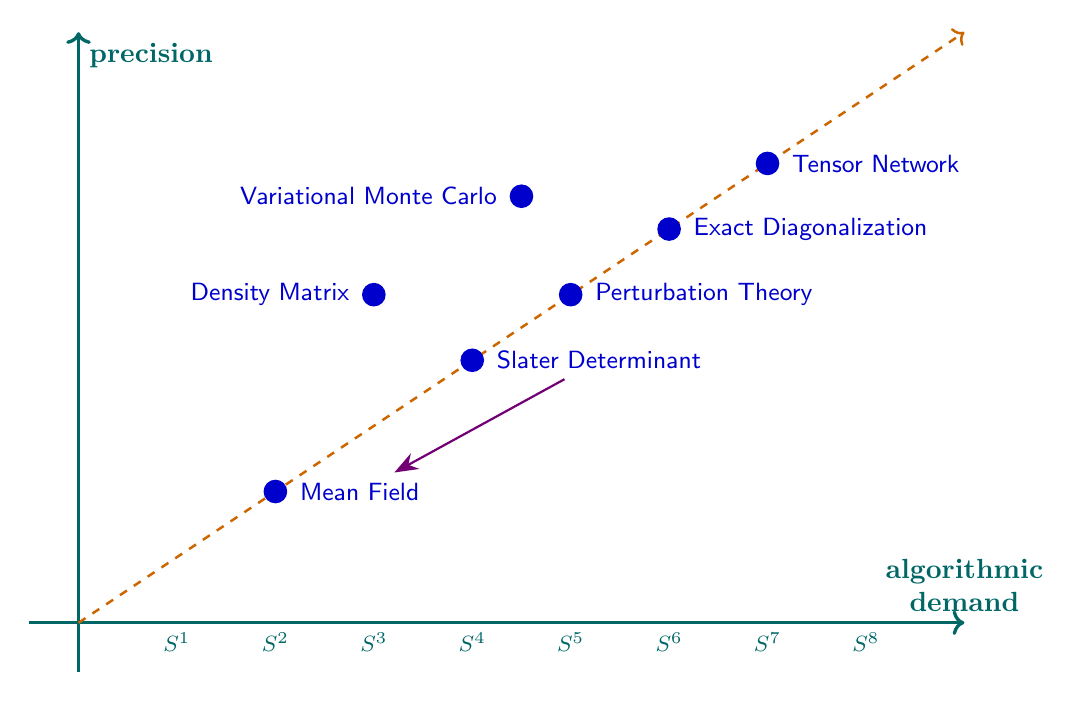
\begin{tikzpicture}[->, thick, align=center, scale=1.25]

  % Axes
  \draw[teal!80!black, line width=1.2pt] (0,-0.5) -- (0,\range*\xyRatio) node[below right, font=\bfseries, teal!80!black] {precision};
  \draw[teal!80!black, line width=1.2pt] (-0.5,0) -- (\range,0) node[above, font=\bfseries, teal!80!black] {algorithmic\\demand};

  % X-ticks
  \foreach \n in {1,...,8}
    \node[below, font=\footnotesize, teal!80!black] at (\n,0) {$S^\n$};

  % Reference diagonal
  \draw[dashed, orange!80!black, line width=0.9pt] (0,0) -- (\range,\range*\xyRatio);

  % Data points (rewritten)
  \foreach \n/\name/\abbr in {2/Mean Field/MF, 4/Slater Determinant/SD, 5/Perturbation Theory/PT, 6/Exact Diagonalization/ED, 7/Tensor Network/TN}
    \fill[blue!80!black] (\n,\xyRatio*\n) circle (\circSize) node[right=1.2ex, font=\sffamily\small, blue!80!black] (\abbr) {\name};

  % Arrow between points
  \draw[thick, violet!90!black, -{Stealth[length=3mm]}] (SD) -- (MF);

  % Additional methods
  \fill[blue!80!black] (3,5*\xyRatio) circle (\circSize) node[left=1.2ex, font=\sffamily\small, blue!80!black] {Density Matrix};
  \fill[blue!80!black] (4.5,6.5*\xyRatio) circle (\circSize) node[left=1.2ex, font=\sffamily\small, blue!80!black] {Variational Monte Carlo};

\end{tikzpicture}
\end{document}